\documentclass{article}
\usepackage{graphicx}
\usepackage[style=ieee]{biblatex} % Establecer el estilo de las referencias como IEEE
\usepackage{xcolor}
\usepackage{hyperref}
\usepackage{titletoc}
\usepackage{adjustbox}
\usepackage[spanish]{babel}

\hypersetup{
    colorlinks=true,
    linkcolor=blue, % Color del texto del enlace
    urlcolor=blue % Color del enlace
}

\usepackage{longtable} % Agrega el paquete longtable

\definecolor{mygreen}{RGB}{0,128,0}

\usepackage{array} % Para personalizar la tabla
\usepackage{booktabs} % Para líneas horizontales de mejor calidad
\usepackage{graphicx} % Paquete para incluir imágenes
\usepackage{float}
\usepackage[section]{placeins}

% Definir márgenes
\usepackage[margin=1in]{geometry}

\renewcommand{\contentsname}{\textcolor{mygreen}{Tabla de Contenidos}}

\begin{document}

\begin{titlepage}
    \centering
    % Logo de la Universidad
    
\includegraphics[width=0.48\textwidth]{logo_universidad.png}
    \par\vspace{2cm}

    % Nombre de la Universidad y detalles del curso
    {\Large \textbf{Universidad Nacional de Colombia} \par}
    \vspace{0.5cm}
    {\large Ingeniería de Sistemas y Computación \par}
    {\large 2025966 Lenguajes de Programación (02)\par}
    \vspace{3cm}

    % Detalles del laboratorio y actividad
    {\large \textbf{Tarea 25} \par}
    {\large Ampliar el analizador léxico para la «selección» agregándole la estructura «while».\par}
    \vspace{3cm}

    % Lista de integrantes
    {\large \textbf{Integrantes:} \par}
    \vspace{0.5cm}
    \begin{tabular}{ll}
    Javier Andrés Tarazona Jiménez & jtarazonaj@unal.edu.co \\
    Eder  José Hernández Buelvas   & ehernandezbu@unal.edu.co \\
    Juan Sebastián Muñoz Lemus     & jumunozle@unal.edu.co   \\
    David Felipe Marin Rosas       & dmarinro@unal.edu.co   \\
    \end{tabular}
    \par\vspace{3cm}

    % Fecha
    {\large 20 de Julio de 2025 \par}
\end{titlepage}

\tableofcontents % Inserta la tabla de contenidos

\newpage % Salto de página para separar la tabla de contenidos del contenido del documento

% Contenido del artículo----------------------------------------------------------

%---------------------------------------------------------------------------------
% Intro --------------------------------------------------------------------------
%---------------------------------------------------------------------------------

\section{Introducción}\label{sec:intr}

El presente documento aborda el desarrollo y comprobación de un analizador léxico elaborado mediante FLEX, una herramienta fundamental en la construcción de esta clase de analizadores. Para ello, se parte de un caso de estudio tomado de la sección 3.23 del libro \textit{Compilers: Principles, Techniques, and Tools} (segunda edición) de Alfred Aho, Monica Lam, Ravi Sethi y Jeffrey Ullman. El propósito principal consiste en ajustar y complementar el código base para que sea capaz de reconocer de forma correcta estructuras de control de flujo como \texttt{while}. Posteriormente, se realizarán diversas pruebas de verificación para confirmar que la implementación identifica y procesa cada componente léxico según lo previsto.

%---------------------------------------------------------------------------------
% Marco Teórico ------------------------------------------------------------------
%---------------------------------------------------------------------------------

\section{Marco Teórico}\label{sec:marc}

\subsection*{Procesadores de Lenguaje}

Los procesadores de lenguaje son programas diseñados para interpretar, transformar o ejecutar instrucciones escritas en un lenguaje de programación. Entre ellos destacan los compiladores, los intérpretes y los sistemas híbridos, cada uno con métodos y propósitos específicos.

\subsection*{Compiladores}

Un compilador traduce un programa fuente a un programa equivalente en otro lenguaje, generalmente de bajo nivel o código máquina. Durante la compilación, se realiza la detección de errores y la optimización del código para su posterior ejecución. Entre las fases involucradas destacan el preprocesamiento, ensamblaje, vinculación y carga, que aseguran que el resultado final sea ejecutable en la plataforma destino.

\subsection*{Intérpretes}

A diferencia del compilador, un intérprete ejecuta directamente las instrucciones del código fuente en tiempo de ejecución. Esta característica permite diagnósticos de errores más detallados, aunque con una menor velocidad de ejecución comparada con programas compilados.

\subsection*{Procesadores Híbridos}

Algunos lenguajes adoptan un enfoque intermedio, generando primero un código intermedio —como el bytecode en Java— que luego es interpretado o compilado dinámicamente mediante técnicas como la compilación JIT (Just-In-Time), mejorando el rendimiento en tiempo de ejecución.

\subsection*{Estructura de un Compilador}

Un compilador se divide conceptualmente en dos etapas: análisis y síntesis.  
\textbf{El análisis} descompone el código fuente en componentes básicos, detecta errores y construye una representación intermedia. Dentro de esta fase, destacan:
\begin{itemize}
    \item \textbf{Análisis léxico:} Identifica lexemas y los convierte en tokens.
    \item \textbf{Análisis sintáctico:} Organiza los tokens en estructuras gramaticales.
    \item \textbf{Análisis semántico:} Verifica la coherencia de las operaciones.
\end{itemize}

\textbf{La síntesis} genera el código objetivo a partir de la representación intermedia, realizando optimizaciones y adaptando la salida al sistema donde se ejecutará.

\subsection*{Análisis Léxico}

El análisis léxico es la fase inicial de un compilador. Su función es leer el flujo de caracteres del programa y agruparlos en unidades significativas llamadas tokens, eliminando elementos irrelevantes como espacios o comentarios. Cada token encapsula información necesaria para las etapas de análisis sintáctico y semántico.

\subsection*{FLEX}

FLEX es una herramienta que automatiza la creación de analizadores léxicos. A partir de una descripción de patrones, genera código capaz de reconocer tokens, facilitando el desarrollo de compiladores y otros sistemas de procesamiento de texto.

\subsection*{Expresiones y Definiciones Regulares}

Para reconocer patrones léxicos, se emplean expresiones regulares, que describen conjuntos de cadenas válidas. Operaciones como la concatenación, alternación o repetición permiten definir patrones complejos. Las definiciones regulares permiten simplificar y reutilizar estos patrones, evitando redundancia y facilitando la lectura y mantenimiento del analizador.

\subsection*{Bucle While}

El bucle \texttt{while} constituye una estructura de control esencial en numerosos lenguajes de programación. Su propósito es ejecutar repetidamente un conjunto de instrucciones mientras se cumpla una condición determinada. La evaluación de la condición se realiza antes de cada iteración, asegurando que el bloque de código se ejecute solo cuando la expresión sea verdadera. Esta característica hace que el \texttt{while} sea especialmente útil para procesar entradas dinámicas o repetir operaciones hasta alcanzar un estado deseado, adaptándose así a situaciones en las que el número de iteraciones no se conoce de antemano.

\subsection{Contextualización del problema}

Dentro del diseño de compiladores, el análisis léxico representa la primera etapa encargada de descomponer el código fuente en unidades básicas significativas, llamadas tokens. Herramientas como FLEX simplifican esta tarea al automatizar la generación de analizadores léxicos mediante el uso de patrones definidos con expresiones regulares. Para que un compilador pueda manejar correctamente estructuras de control como el bucle \texttt{while}, es necesario que el analizador léxico identifique este patrón específico junto con otros elementos léxicos del lenguaje, como operadores de comparación, identificadores válidos y cadenas de texto.

Por ello, este proyecto se centra en extender un analizador léxico existente, implementado con FLEX, adaptándolo para reconocer adecuadamente la estructura \texttt{while} junto con sus componentes asociados. De esta forma, se garantiza que el procesador de lenguaje cumpla con los requisitos de un compilador moderno, combinando teoría y práctica en la creación de sistemas capaces de interpretar, transformar y ejecutar instrucciones de manera eficiente.


%---------------------------------------------------------------------------------
% Descripción y Justificación del Problema a Resolver ----------------------------
%---------------------------------------------------------------------------------

\section{Descripción y Justificación del Problema a Resolver}\label{sec:descr}

Este proyecto consiste en extender y adaptar un analizador léxico mediante el uso del generador de analizadores FLEX. En concreto, se modifica un ejemplo propuesto en el texto mencionado, ampliándolo para reconocer la estructura condicional \texttt{while}, operadores de comparación como los que se emplean en el lenguaje C, admitir el guion bajo (\texttt{\_}) como carácter válido en identificadores y gestionar cadenas de texto delimitadas por comillas dobles, incluyendo secuencias de escape para caracteres especiales como las comillas y barras invertidas. Estas ampliaciones buscan garantizar que el programa procese correctamente los nuevos elementos léxicos del lenguaje.

\section*{Justificación}
La práctica con FLEX resulta esencial para estudiantes y profesionales de Ingeniería de Sistemas y Ciencias de la Computación que se interesen en el diseño de compiladores y herramientas relacionadas con el procesamiento de lenguajes. FLEX automatiza la fase de análisis léxico, que constituye la etapa inicial en la construcción de un compilador. Mediante esta actividad se consolidan conocimientos teóricos en un entorno práctico, fortaleciendo la capacidad de adaptar ejemplos de referencia a plataformas de compilación actuales.
\subsection{Objetivo Principal}
El objetivo principal de este trabajo es diseñar, ajustar y validar un analizador léxico empleando la herramienta FLEX, de modo que sea capaz de identificar correctamente estructuras de control como \texttt{while}, operadores de comparación, identificadores con guion bajo y cadenas de texto con manejo de caracteres especiales. Esto permitirá comprobar la funcionalidad del analizador en un contexto de compilación real, asegurando su correcto desempeño al procesar los elementos definidos en el lenguaje de entrada.

%---------------------------------------------------------------------------------
% Diseño de la solución ---------------------------------------------------------
%---------------------------------------------------------------------------------

\section{Diseño de la solución}\label{sec:dis}

La solución es propuesta como una herramienta didáctica y de experimentación, orientada a facilitar la comprensión y puesta en práctica de conceptos clave relacionados con los analizadores léxicos. La aplicación brinda un entorno accesible para crear, modificar, compilar y ejecutar analizadores léxicos construidos con FLEX, haciendo énfasis en el reconocimiento de estructuras fundamentales como \texttt{if}, \texttt{while}, \texttt{then}, \texttt{else}, \texttt{id}, \texttt{number}, operadores relacionales (\texttt{relop}) y cadenas de texto delimitadas por comillas dobles (\texttt{doubleq}).

Entre las funcionalidades destacadas se encuentra la gestión centralizada de constantes léxicas, lo que permite mantener organizadas las palabras reservadas y categorías definidas, promoviendo la escalabilidad y el mantenimiento del código generado. Además, se incorpora un sistema de compilación automática que combina FLEX y GCC, simplificando la conversión del código fuente en un ejecutable funcional, optimizando así el proceso de validación y prueba del analizador.

El diseño sigue un esquema modular que divide las tareas en bloques funcionales independientes:

\begin{enumerate}
    \item \textbf{Módulo de Edición de Código:} Brinda al usuario un espacio para redactar o ajustar el archivo fuente FLEX. Incluye mecanismos de verificación básica de la sintaxis y comprobación de la correcta declaración de constantes.
    \item \textbf{Módulo de Compilación:} Encargado de coordinar la generación del código intermedio en C a partir del archivo FLEX y su posterior compilación usando GCC, asegurando la creación de un ejecutable listo para pruebas.
\end{enumerate}

\subsection{Metodología}

Para llevar a cabo el desarrollo y validación de la aplicación, se plantea una metodología dividida en etapas:

\begin{enumerate}
    \item \textbf{Análisis y Planificación:} Se revisa la estructura del analizador original y se identifican los elementos que requieren extensión, como el soporte para nuevas palabras clave, operadores y cadenas de texto.
    \item \textbf{Implementación del Código FLEX:} Se redacta y ajusta el archivo fuente FLEX, integrando definiciones y expresiones regulares que describan cada patrón léxico a reconocer.
    \item \textbf{Pruebas de Compilación:} Se automatiza el proceso de conversión del archivo FLEX a C y su compilación con GCC, garantizando que el ejecutable se genere sin errores.
    \item \textbf{Verificación Funcional:} Se realizan casos de prueba para confirmar que el analizador detecta correctamente los tokens definidos, prestando especial atención a la estructura \texttt{while} y la correcta interpretación de operadores y cadenas.
    \item \textbf{Documentación y Validación Final:} Se elabora la documentación que describe el funcionamiento de la herramienta, sus componentes y la evidencia de que cumple con los objetivos planteados.
\end{enumerate}

%---------------------------------------------------------------------------------
% Código Fuente ---------------------------------------------------------
%---------------------------------------------------------------------------------

\section{Código Fuente}\label{sec:cod}

El código fuente de esta tarea se encuentra adjunto en el buzón 
(25 Muñoz Lemus Juan Sebastian 02.zip)
y disponible en el repositorio GitHub del proyecto:

\begin{center}
\url{URL}
\end{center}

%---------------------------------------------------------------------------------
% Manual Usuario ---------------------------------------------------------
%---------------------------------------------------------------------------------

\section{Manual Usuario}\label{sec:man_u}

A continuación se detalla una guía básica para instalar las herramientas necesarias y ejecutar correctamente el analizador léxico desarrollado:

\subsection*{Instalación de Herramientas}

Para comenzar, es indispensable contar con \texttt{FLEX}, \texttt{MinGW} y \texttt{Bison}. Se recomienda seguir las instrucciones proporcionadas en el manual de la tarea 23 para completar la instalación de cada componente.

\subsection*{Obtención del Código Fuente}

\begin{enumerate}
    \item Acceda a este enlace
    \item Descargue el archivo Tarea25.l
    \item Una vez descargado, guarde el archivo en una carpeta.
\end{enumerate}

\subsection*{Ejecución en el Entorno de Desarrollo}

\begin{enumerate}
    \item Abra su editor de código.
    \item Desde el editor, seleccione la carpeta que contiene el archivo \texttt{Tarea25.l}.
    \item Abra una terminal en el mismo entorno.
    \item Compile el archivo fuente ejecutando el siguiente comando:
    \begin{verbatim}
flex Tarea25.l
    \end{verbatim}
    \item Genere el ejecutable utilizando \texttt{gcc} con el comando:
    \begin{verbatim}
gcc lex.yy.c -lfl
    \end{verbatim}
    \item Verifique que el proceso finalice sin errores y ejecute el programa resultante para probar el analizador.
\end{enumerate}

%---------------------------------------------------------------------------------
% Manual Técnico ---------------------------------------------------------
%---------------------------------------------------------------------------------

%---------------------------------------------------------------------------------
% Experimentación ---------------------------------------------------------
%---------------------------------------------------------------------------------

\section{Experimentación}\label{sec:exp}

\section*{Experimentación}

Para comprobar la funcionalidad del analizador léxico, se siguió un procedimiento experimental dividido en tres etapas principales. En primer lugar, se tomó como base el código de la tarea anterior y se realizaron ajustes para ampliar su alcance:

\begin{enumerate}
    \item \textbf{Etapa 1: Ampliación de palabras clave y operadores} \\
    Se incorporó la palabra clave \texttt{while} para permitir la detección de bucles de repetición. Asimismo, se redefinieron los operadores relacionales para adaptarlos a la sintaxis de C, integrando símbolos como \texttt{<}, \texttt{<=}, \texttt{>}, \texttt{>=}, \texttt{==} y \texttt{!=}.

\begin{verbatim}
while { return (WHILE); }
 "<" {yylval = LT; return (RELOP); }
 "<=" {yylval = LE; return (RELOP); }
 "==" {yylval = EQ; return (RELOP); }
 "!=" {yylval = NE; return (RELOP); }
 ">" {yylval = GT; return (RELOP); }
 ">=" {yylval = GE; return (RELOP); }        
\end{verbatim}
    
\item \textbf{Etapa 2: Inclusión del guion bajo en identificadores} \\
Se modificó la definición de identificadores para admitir el carácter guion bajo (\texttt{\_}), posibilitando la creación de nombres de variables o etiquetas más flexibles y alineados con las prácticas habituales de programación.

\begin{verbatim}
id {letter}({letter}|{digit}|_)   
\end{verbatim}
    
\item \textbf{Etapa 3: Manejo de cadenas de texto} \\
Se añadió soporte para reconocer cadenas delimitadas por comillas dobles. Para contemplar caracteres especiales dentro de estas cadenas, se implementó el uso de secuencias de escape para comillas internas y barras invertidas.
\begin{verbatim}
doubleq.*doubleq { yylval = (int) installString(); return (STRING); }       
\end{verbatim}
\end{enumerate}

Tras aplicar estas modificaciones, se procedió a compilar y ejecutar el archivo FLEX utilizando los comandos:
\begin{verbatim}
flex Tarea25.l
gcc lex.yy.c -lfl
\end{verbatim}
\begin{figure}[H]
    \centering
    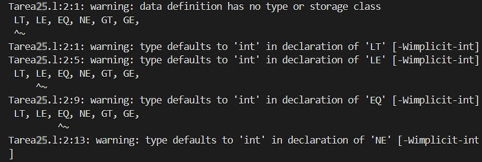
\includegraphics[width=0.7\linewidth]{image.jpg}
\end{figure}

\subsection{Análisis de resultados}

Durante la fase de ejecución se detectaron varios problemas que impidieron la generación correcta del analizador léxico. Entre los mensajes de advertencia figuraron declaraciones implícitas para constantes y tokens como \texttt{LT}, \texttt{LE}, \texttt{EQ}, \texttt{NE}, \texttt{GT}, \texttt{GE} y las palabras clave \texttt{IF}, \texttt{THEN}, \texttt{ELSE}, \texttt{ID}, \texttt{NUMBER}, \texttt{RELOP} y \texttt{WHILE}. 

Adicionalmente, se reportaron errores relacionados con identificadores y funciones no definidos, tales como \texttt{WHILE}, \texttt{yylval}, \texttt{installID}, \texttt{installString} e \texttt{installNum}. También se identificaron fallos potenciales por la ausencia de la definición adecuada de la función \texttt{yywrap} y posibles omisiones en la inclusión de cabeceras o archivos complementarios que contienen estas declaraciones.

\subsection{Conclusiones }

A partir de los resultados obtenidos se concluye que, si bien se avanzó en la ampliación de capacidades del analizador léxico, persisten aspectos de configuración y declaración que deben ser revisados. Los principales inconvenientes se relacionan con la falta de definición de constantes, tokens y funciones de apoyo indispensables para la correcta compilación del programa.

\section{Referencias}
\renewcommand{\refname}{}
\begin{thebibliography}{9}
\bibitem{1}
Aho, A. V., Lam, M. S., Sethi, R., \& Ullman, J. D. (2007). \textit{Compilers: Principles, Techniques, and Tools} (2nd ed.). Pearson Education.
\bibitem{2}
Appel, A. W., \& Palsberg, J. (2004). \textit{Modern Compiler Implementation in Java} (2nd ed.). Cambridge University Press.
\bibitem{3}
Westes, B. (n.d.). \textit{flex: The fast lexical analyzer}. GitHub. Retrieved December 13, 2024, from \url{https://github.com/westes/flex}

\end{thebibliography}

\end{document}